\documentclass{article}
\usepackage{tikz}
\usetikzlibrary{automata, positioning}

\begin{document}

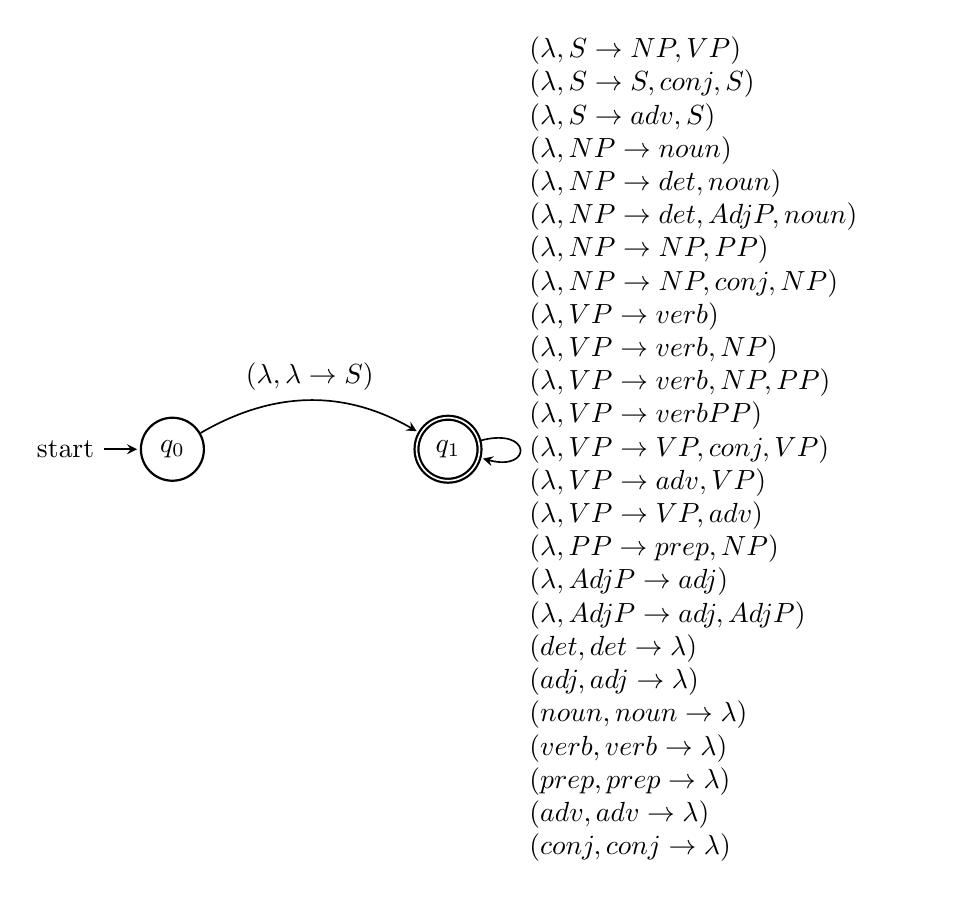
\begin{tikzpicture}[->, >=stealth, shorten >=1pt, auto, node distance=3.5cm, semithick]
  \tikzstyle{every state}=[draw=black, thick, minimum size=8mm]

  % States
  \node[state, initial] (q0) {$q_0$};
  \node[state, accepting, right of=q0] (q1) {$q_1$};

  % Transitions

  \path (q0) edge[bend left] node {
    $(\lambda, \lambda \rightarrow S)$
  } (q1);

\path (q1) edge[loop right] node[text width=5cm, align=left] {
  $(\lambda, S \rightarrow NP, VP)$\\
  $(\lambda, S \rightarrow S, conj, S)$\\
  $(\lambda, S \rightarrow adv, S)$\\
  $(\lambda, NP \rightarrow noun)$\\
  $(\lambda, NP \rightarrow det, noun)$\\
  $(\lambda, NP \rightarrow det, AdjP, noun)$\\
  $(\lambda, NP \rightarrow NP, PP)$\\
  $(\lambda, NP \rightarrow NP, conj, NP)$\\
  $(\lambda, VP \rightarrow verb)$\\
  $(\lambda, VP \rightarrow verb, NP)$\\
  $(\lambda, VP \rightarrow verb, NP, PP)$\\
  $(\lambda, VP \rightarrow verb PP)$\\
  $(\lambda, VP \rightarrow VP, conj, VP)$\\
  $(\lambda, VP \rightarrow adv, VP)$\\
  $(\lambda, VP \rightarrow VP, adv)$\\
  $(\lambda, PP \rightarrow prep, NP)$\\
  $(\lambda, AdjP \rightarrow adj)$\\
  $(\lambda, AdjP \rightarrow adj, AdjP)$\\
  $(det, det \rightarrow \lambda)$\\
  $(adj, adj \rightarrow \lambda)$\\
  $(noun, noun \rightarrow \lambda)$\\
  $(verb, verb \rightarrow \lambda)$\\
  $(prep, prep \rightarrow \lambda)$\\
  $(adv, adv \rightarrow \lambda)$\\
  $(conj, conj \rightarrow \lambda)$  
} (q1);

\end{tikzpicture}

\end{document}
